\section{Proposed Method}\label{sec:method}
In this section, we introduce a method for detecting different forms of face spoofing attacks. The method comprises three main steps: \emph{low-level descriptor extraction}, \emph{mid-level descriptor extraction}, and \emph{classification}. Fig.~\ref{fig:method_overview} \minor{illustrates} these steps, which we explain in details in the following sections.

We designed the algorithm based on the fact that synthetic biometric samples contain noise and artifacts generated during their manufacture and recapture that are different \minor{from} any pattern found in real biometric samples. According to Tan et al.~\cite{Tan:ECCV:2010} and M\"{a}\"{a}tt\"{a} et al.~\cite{Maatta:IJCB:2011}, there is a deterioration of the facial information and, consequently, a loss of some high frequency components during the manufacture of photographs to be used in spoofing attacks. In our prior work~\cite{Pinto:SIBGRAPI:2012}, we highlighted the fact that there is a significant increase of the low frequency components due to the blurring effect added during the recapture process of the biometric sample displayed in tablets, smartphones and laptop screens. Besides the blurring effect, other artifacts are added \redmark{such as flickering, Moir\'e patterns, and banding effect~\cite{Beach:PP:2008}}.

\redmark{These facts motivated us to propose a solution that takes advantage of the noise and artifacts contained on such fake biometric samples, which heretofore we refer to as a noise signature. We perform a Fourier analysis of the noise signature to capture the information encoded in the frequency, phase and amplitude of the component sinusoids~\cite{Smith:SEG:1997}. In this paper, we use Fourier spectrum to quantify the following artifacts:}
%
\begin{itemize}
	\item \textit{\redmark{blurring artifact}:} In both the production and recapture processes, inevitably we have a decrease in the details of biometric samples due to re-quantization of the original signal. This reduction of details is reflected in the increase of low frequency components and can be observed in the Fourier domain;
	
	\item \textit{flickering effect:} It corresponds to the horizontal and vertical lines equally spaced that appear during the recapture process of the samples shown to the acquisition sensor with the display device. When this artifact appears in biometric samples, there are peak lines at abscissa and ordinate axes of the Fourier spectrum when the display device is aligned with the acquisition sensor;
	
	\item \textit{\redmark{Moir\'e pattern}:} They are irregular patterns \redmark{that can appear} when a display device is used to perform an attempted attack. As a result, we also have the appearance of peaks in different locations in the Fourier spectrum depending on the {frequency and direction of the sinusoid in the spatial domain}~\cite{Smith:SEG:1997}.
\end{itemize}

The novelty of our solution is in the two-tier low and mid-level characterization scheme, called time-spectral visual words, that captures patterns present in such noise signatures useful to reveal spoofing attacks. For this, we extract \redmark{temporal-spectral descriptors} from the noise signature transformed to the frequency domain and create a mid-level representation for them using the concept of visual codebooks~\cite{Sivic:ICCV:2003,Avila:ICIP:2011}. Visual codebooks are a method for constructing mid-level representations widely employed in several applications in pattern recognition and computer vision, \allan{such as object recognition~\cite{Vigo:ICPR:2010}, gesture recognition~\cite{Vela:ICPR:2012}, and information retrieval~\cite{Penatti:PR:2014}, among others}. However, \minor{unlike existing methods, we obtain visual informative features} from the \redmark{noise signature present in the videos} instead of their raw pixels or from objects in the scene. 

\subsection{Low-Level Descriptor Extraction}
In our previous work~\cite{Pinto:SIBGRAPI:2012}, we found that the noise signal is an important source for low-level discriminative features for spoofing detection. When working with the noise signal and discarding the video content, \redmark{we minimize possible negative impacts on the \allan{method performance}. Next, we present the \allan{steps} of the proposed method to compute the low-level descriptors.} 

%\todo{me parece forte falar que a remocao do conteudo reduz o impacto da iluminacao, uma vez que a iluminacao impacta as frequencias espaciais da imagem, talvez tirar a parte do such as e deixar geral para evitar algum comentario do revisor}

\subsubsection{Calculation of the Residual Noise Videos}
The low-level representation of the videos is computed through the spectrum analysis of the noise signal in the frequency domain. To isolate the noise signal of a given video $V$, we filter a copy of $V$ using a Gaussian filter with mean $\mu$, std. $\sigma$, and kernel size $k \times k$ to remove the high frequency components, generating a filtered video. Then, we perform a subtraction operation between the input video and its filtered version, generating a new video, called \redmark{Residual Noise Video ($V_{RN}$)}: 
\begin{equation}
V_{RN}^{(t)} = V^{(t)} - h(V^{(t)}) \quad \forall \textrm{ \textit{t} } \in \mathit{T} =\{1, 2, \ldots, t\},
\label{eq:ruido}
\end{equation}
\noindent where $V^{(t)} \in \mathbb{N}^2$ is the $t$-th frame of $V$ and $h$ is a filter whose impulse response is a Gaussian function.

\subsubsection{Calculation of the Fourier Spectrum Videos}
After calculating the residual noise videos, we can analyze the noise pattern and possible artifacts contained in the biometric samples by applying the 2D Discrete Fourier Transform to each frame of the \allan{$V_{\text{RN}}$} using Eq.~\ref{eq:dft}. In this work, we evaluate two important characteristics of the noise signal in the frequency domain, the magnitude and phase of the signal. The analysis of these two characteristics is performed by calculating the magnitude spectrum (Eq.~\ref{eq:mag_spectrum}) and phase spectrum (Eq.~\ref{eq:phase_spectrum}), with the origin at the center of the frame. In both cases, the result is a Fourier spectrum video.

\begin{small}
\begin{align}
\mathcal{F}{(V_{\text{RN}}(x,y))} &\equiv F(v, u) \\
F(v, u) &= \sum_{x=0}^{M-1}{\sum_{y=0}^{N-1}{V_{\text{RN}}(x,y)e^{-j2\pi[(vx/M) + (uy/N)]}}} \label{eq:dft} \\
|{F}{(v, u)}| &= \sqrt{\mathcal{R}{(v, u)}^{2} + \mathcal{I}{(v, u)}^{2}} \\
V_{\text{MS}}{(v, u)} &= \log(1 + |{F}{(v, u)}|) \label{eq:mag_spectrum} \\
V_{\text{PS}}(v, u) &= \arctan{\left(\frac{\mathcal{I}{(v, u)}}{\mathcal{R}{(v, u)}}\right)} \label{eq:phase_spectrum}
\end{align}
\end{small}

From the Fourier spectrum video, we can extract spectral and temporal information relevant to the spoofing attack detection. In the case of the spectral information, we need to capture peaks present in the central region caused by artifacts that reduce some details in the scene (e.g., skin marking, edge information) such as blurring effect, defocus, and printing artifacts and peaks present in the peripheral region of the frame caused mainly by artifacts such as the banding effect and Moir\'e pattern, which appear during the recapture of the biometric information during an attack. 

\redmark{Figs.~\ref{fig:noise_spectra_real1} and~\ref{fig:noise_spectra_attack1} show an attempt to depict the temporal disturbances added to the biometric samples during attacks. In this example,  we extract the first ten consecutive frames of an attack video and of a valid video for the same client, and calculate their respective magnitudes spectra from the residual noise video. In addition, Fig.~\ref{fig:noise_spectra_attack2} shows examples in which we have frames extracted from valid access videos (a) and spoof attack videos (b-c). In this figure, we aim at showing the Moiré and blurring effects found in attempted attacks performed with a mobile device. The blurring effect is present in the magnitude spectrum with an increase of the low frequency components, whereas the Moiré effect is present in the magnitude spectrum with peaks in the horizontal center region of the frames. It is hard to find a direct mapping of the effects to the phase spectra, but we can see clearly that there are disturbances in the phase spectra calculated from attempted attack frames when compared to phase spectra extracted from valid access frames.}

\minor{It is important to remark that} we are not proposing a method \minor{for capturing} each of the artifacts separately. We believe that the presence of one or more artifacts \minor{causes} disturbances in the frequency components in the Fourier domain and the proposed method aims at describing and capturing this disturbance in space and time.
%
\begin{figure*}[!htb]
	\centering
	\subfloat[Original frames]{\includegraphics[width=0.75\textwidth]{./original_train/real/client004_session01_webcam_authenticate_controlled_1.png}}\\
	\subfloat[Residual noise frames]{\includegraphics[width=0.75\textwidth]{./ritmo_noisetrain/real/client004_session01_webcam_authenticate_controlled_1.png}}\\
	\subfloat[Magnitude spectra]{\includegraphics[width=0.75\textwidth]{./ritmo_spectrain/real/client004_session01_webcam_authenticate_controlled_1.png}}
	\caption{(a) Original frames extracted from a valid access video, (b) their respective \allan{residual noise frames} and (c) magnitude spectra.
	\label{fig:noise_spectra_real1}}
\end{figure*}
%
\begin{figure*}[htb]
	\centering
	\subfloat[Original frames]{\includegraphics[width=0.75\textwidth]{./original_train/attack/hand/attack_mobile_client004_session01_mobile_photo_controlled.png}}\\
	\subfloat[Residual noise frames]{\includegraphics[width=0.75\textwidth]{./ritmo_noisetrain/attack/hand/attack_mobile_client004_session01_mobile_photo_controlled.png}}\\
	\subfloat[Magnitude spectra]{\includegraphics[width=0.75\textwidth]{./ritmo_spectrain/attack/hand/attack_mobile_client004_session01_mobile_photo_controlled.png}}
	\caption{(a) Original frames extracted from an attempted attack video, (b) their respective \allan{residual noise frames} and (c) magnitude spectra.
	\label{fig:noise_spectra_attack1}}
\end{figure*}
%
\begin{figure*}[!htp]
	\centering
	\subfloat[Examples of a frame extracted from valid access video]{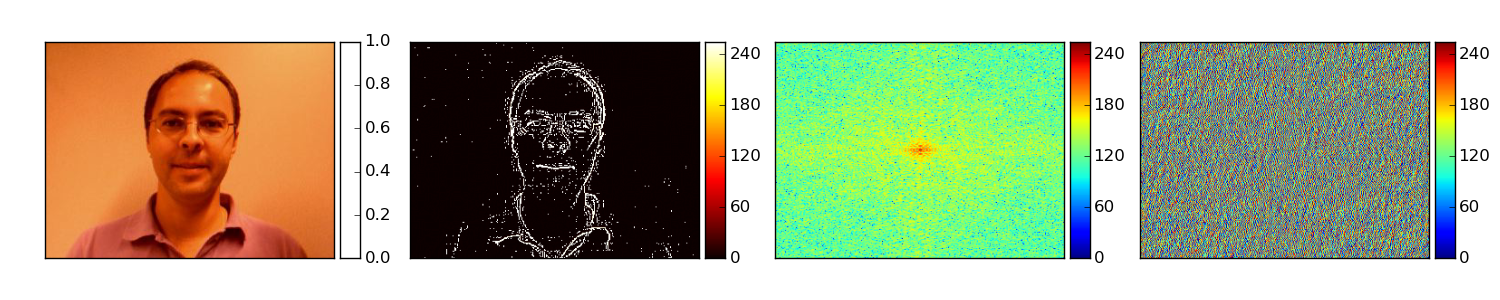
\includegraphics[width=0.68\textwidth]{client001_session01_webcam_authenticate_controlled_1_000.png}}\\
	\subfloat[Examples of frames extracted from a mobile-attack videos. We highlighted the Moiré effect with yellow circle in the original image and its respective residual noise frame. The arrows on the magnitude spectrum indicate the effect of the Moiré effect over Fourier spectrum]{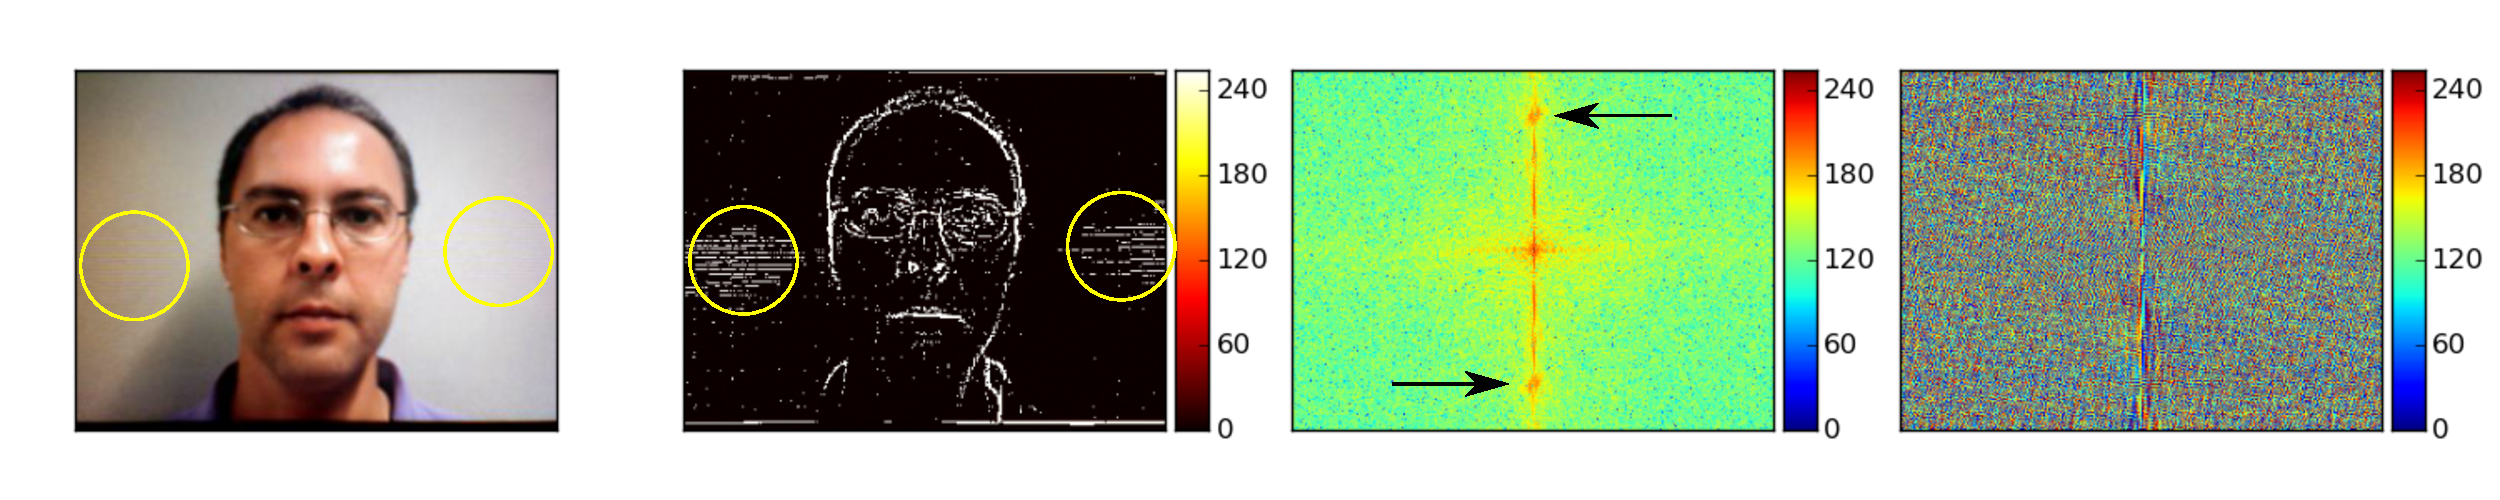
\includegraphics[width=0.68\textwidth]{attack_mobile_client001_session01_mobile_photo_controlled_000.pdf}}\\
	\subfloat[Examples of frames extracted from a mobile-attack videos. In this frame, we show a blurring effect in the original image and its effect in the residual noise frame. The arrows on the magnitude spectrum show the impact of this effect over Fourier spectrum]{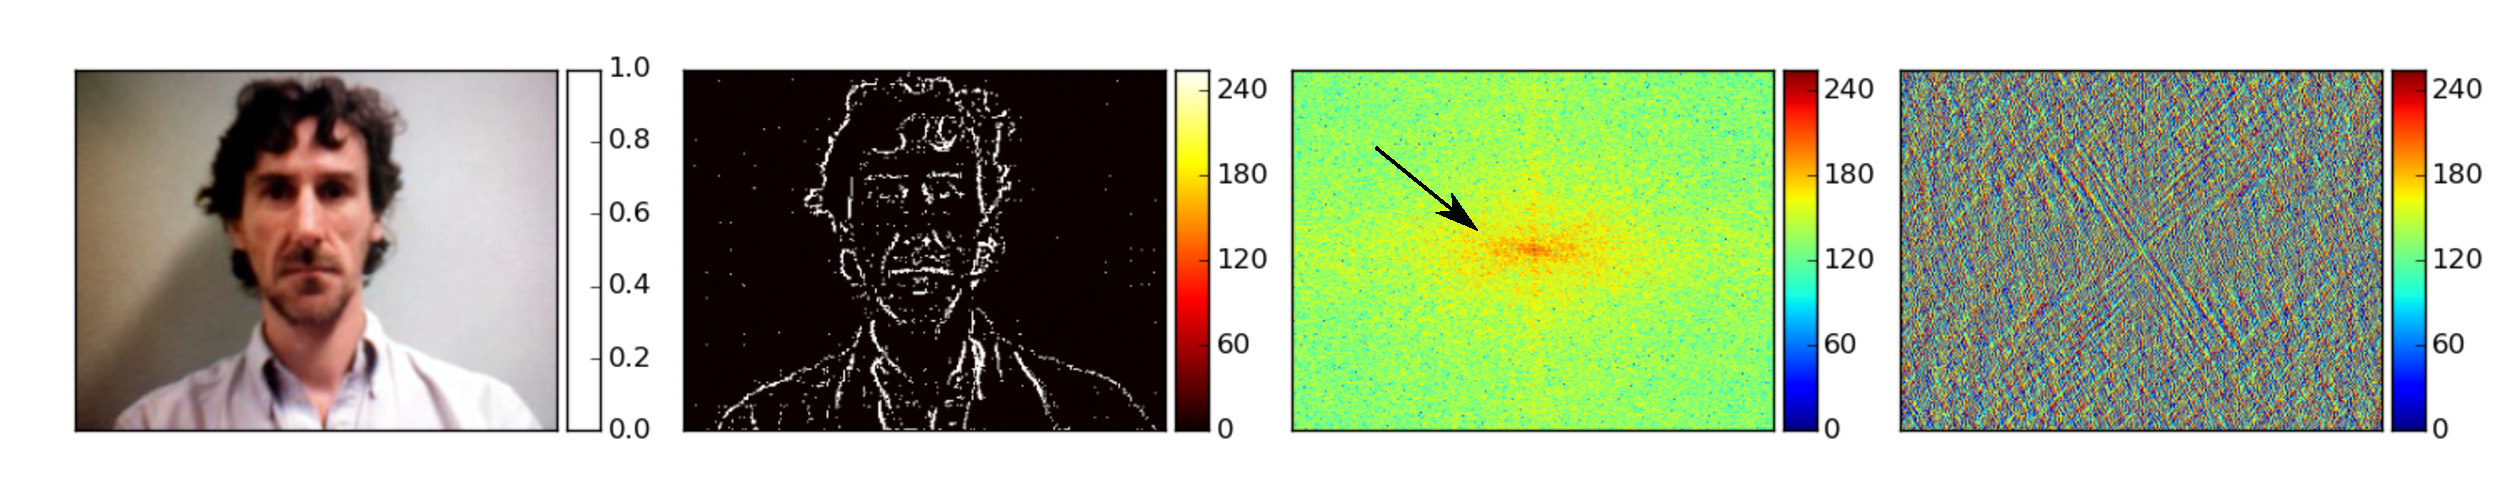
\includegraphics[width=0.68\textwidth]{attack_mobile_client011_session01_mobile_photo_controlled_009.pdf}}\\
	\caption{Examples of valid access and attempted attack videos. The first column shows the original frame extracted from a video and the second column shows the \allan{residual noise frame} calculated from the original frames. Finally, the third and fourth columns show the magnitude and phase spectrum, respectively. Note that the phase spectra calculated from valid access frames are different from attempted attack frames.\label{fig:effects}}
	\label{fig:noise_spectra_attack2}
\end{figure*}
%
%%
%\begin{figure*}[!ht]
%\centering
%\subfloat[Magnitude spectra calculated from a valid access video.]{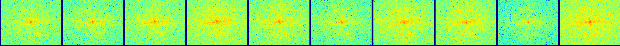
\includegraphics[width=0.82\textwidth]{./figures/temporal/client020_session01_webcam_authenticate_controlled_2.png}}\hspace{1.0mm}
%%
%\subfloat[Magnitude spectra calculated from a spoof attack video.]{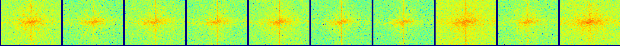
\includegraphics[width=0.82\textwidth]{./figures/temporal/attack_mobile_client020_session01_mobile_video_controlled.png}}
%\caption{Examples of the first ten magnitude spectra calculated from a \textbf{valid access} video (a) and a \textbf{spoof attack} video (b).}
%\label{fig:tempartifacts}
%\end{figure*}
%%
%\begin{figure*}[!ht]
%\centering
%\subfloat[Examples of frames extracted from valid access videos for two users on Replay-Attack dataset.]{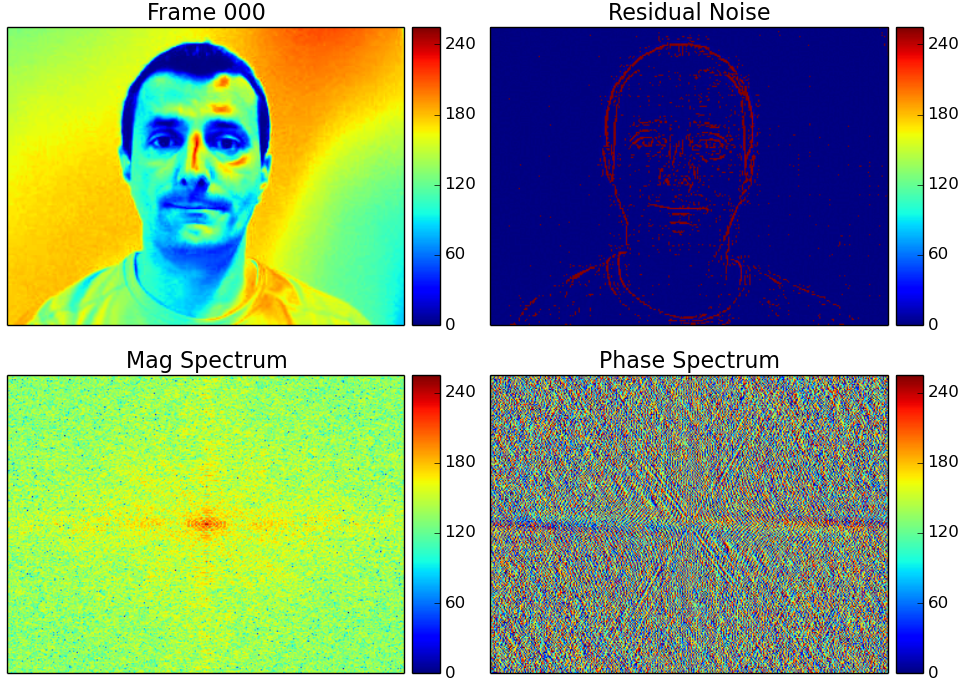
\includegraphics[width=0.39\textwidth]{./figures/artifacts/client026_session01_webcam_authenticate_controlled_1_000.png}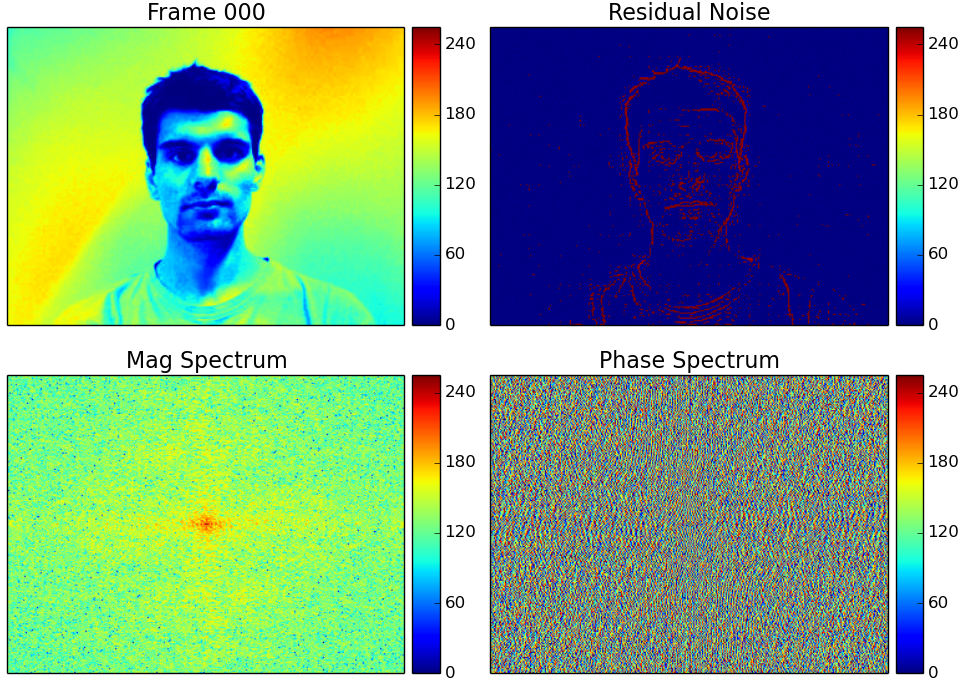
\includegraphics[width=0.39\textwidth]{./figures/artifacts/client020_session01_webcam_authenticate_controlled_1_000.png}}\\
%%
%\subfloat[Example of frame extracted from a spoof attack video.]{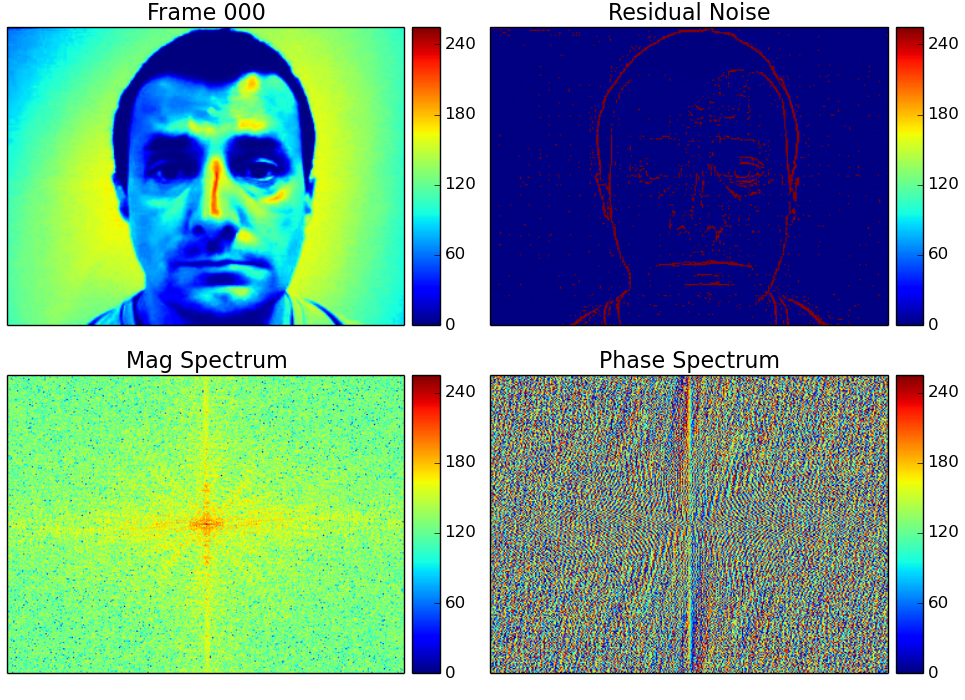
\includegraphics[width=0.39\textwidth]{./figures/artifacts/attack_highdef_client026_session01_highdef_video_controlled_000.png}}\hspace{0.5mm}
%\subfloat[Example of frame extracted from a spoof attack video.]{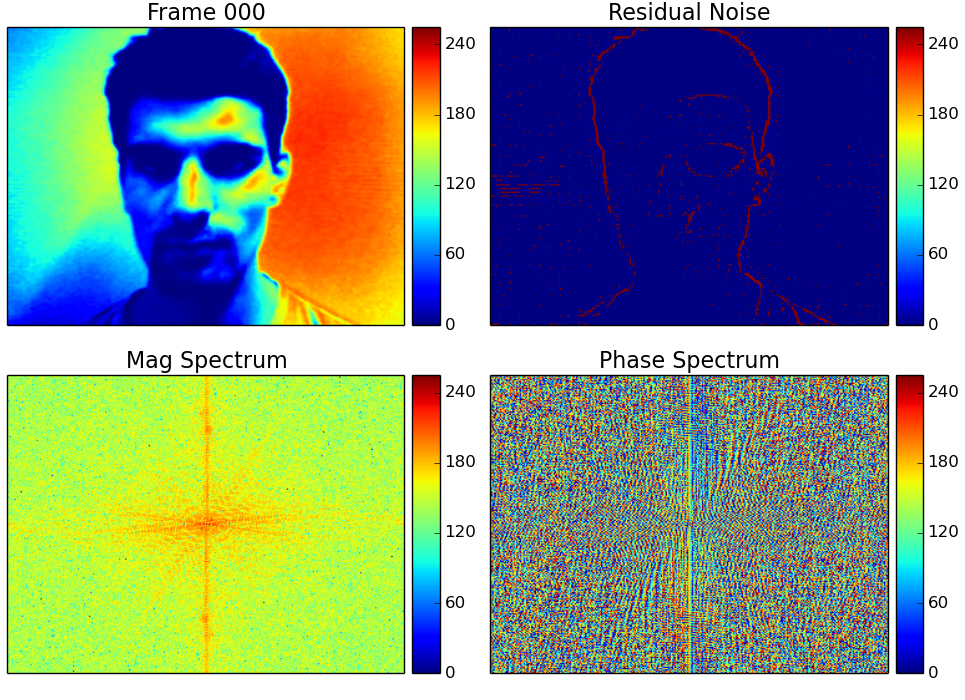
\includegraphics[width=0.39\textwidth]{./figures/artifacts/attack_mobile_client020_session01_mobile_video_controlled_000.png}}
%\caption{Examples of video frames of \textbf{valid access} videos (a) and \textbf{spoof attack} videos (b-c). Fig.\ref{fig:artifacts}(c)~and~(d) illustrate examples of blurring effect, characterized by the loss of details in the face region  and Fig.\ref{fig:artifacts}(b)~and~(c) show flickering effects, characterized by the appearance of collinear points (b) and horizontal traces (c), both in the background.}
%\label{fig:artifacts}
%\end{figure*}

\subsubsection{Computation of the time-spectral descriptor}
Due to the dynamics involved in the appearance of artifacts and noise in the synthetic biometric samples \minor{and the} spectral information, the temporal information becomes important to detect spoofing attacks. Therefore, we design a feature descriptor that gathers temporal and spectral information from an input video. We extract $n$ temporal cubes of size of $w \times h \times t$ \minor{(blocks of size $w \times h$ of $t$ frames) from the Fourier spectrum video}. The idea of temporal cubes has been somewhat explored to quantify temporal information in other tasks in computer vision~\cite{Klaeser:BMVA:2008,Alon:TPAMI:2009,Ren:PR:2009}. In all cases, it always boils down to designing important discriminative features for capturing the event of interest. In this paper, we design new ideas for spoofing detection.

%The extracted temporal cubes are hereinafter named as time-spectral features, which contain information about the temporal behavior of the frequency components that form the input video. 

\minor{The computation of the measure over temporal cubes can be performed on each frame separately, hereinafter referred to as spatial measures, or between consecutive frames, hereinafter referred to spatio-temporal measures. Examples of spatial measures that can be used are energy and entropy of the signal, which quantify the signal size and amount of information, respectively. As examples of spatial-temporal measures, we can mention correlation and mutual information, which are applied to measure dependence between consecutive frames. At the end of this process, we have a set of $n$ time-spectral descriptors of $t$ dimensions, for each video. As spatio-temporal measures are applied on consecutive frames, this process yield $n$ time-spectral descriptors of $(t-1)$ dimensions each.}

\subsection{Mid-Level Descriptor Extraction}
To find a robust representation for the low-level feature descriptors, with less sensitivity to the intra- and extra-class variations, we use the Bag-of-Visual-Word (BoVW) model~\cite{Sivic:ICCV:2003}, which maps the low-level features onto a more discriminative mid-level representation. Methods based on the BoVW model can be understood in the following steps: \minor{visual} codebook generation, coding, and pooling.

\subsubsection{Visual Codebook Generation}
The generation of the visual codebook consists in the selection of time-spectral descriptors that are more frequent and representative considering all descriptors extracted from training videos. The selected descriptors, called time-spectral visual words, form the visual codebook. The selection can be performed using two strategies: (1) random selection, whereby all descriptors are pooled and $m$ visual words are randomly chosen using a uniform distribution; or (2) selection via clustering (e.g., $k$-means) whereby all descriptors undergo a clustering process and the $m$ centroids found by the algorithm are used to form the visual codebook. In both cases, we end up with a single visual codebook, which is used to encode the low-level time-spectral descriptors from videos.

\minor{Instead of pooling all descriptors extracted from videos into a training set to build a single visual codebook, we can build class-based visual codebooks. When creating class-based visual codebooks, we consider the use of valid access and attempted attack video descriptors separately in order to find codebooks in each class. For each class-based codebook, we use the same procedures described above for a single visual codebook creation. The two visual codebooks are concatenated to create the final codebook.}

\subsubsection{Coding}
The coding process performs a pointwise transformation of the low-level descriptors into another representation~\cite{Boureau:CVPR:2010}. There are several strategies for coding \minor{being} the hard and soft assignments the most common. Given a visual codebook and a low-level descriptor, the hard assignment transforms such descriptor into a binary vector with only one nonzero coefficient representing the visual word closest to it. The \minor{soft assignment}~\cite{Gemert:ECCV:2008}, in turn, gives a real valued vector that represents the descriptor as a linear combination of the visual words of the codebook, whose coefficients give an associativity degree between the descriptor and the visual words of the codebook~\cite{Liu:ICCV:2011}. In this paper, we evaluate these two strategies for coding the low-level descriptors.

\subsubsection{Pooling}
The pooling process aims at summarizing the information contained in the set of $n$ mid-level feature descriptors extracted from an input video into only one feature descriptor to obtain its final representation. In the literature, we have two common techniques to do that, known as sum-pooling (Eq.~\ref{eq:sum_pooling}) and max-pooling (Eq.~\ref{eq:max_pooling}). In this paper, we evaluate these two strategies, as well.
%
\begin{eqnarray}
\begin{small}
	v_{i}^{(j)} = \sum_{i=1}^{n}{u_{i}^{(j)}} \quad \forall \textrm{ \textit{j} } \in \{1, 2, \ldots, m\}
\label{eq:sum_pooling}
\end{small}
\end{eqnarray}
%
\begin{eqnarray}
\begin{small}
	v_{i}^{(j)} = \mathtt{max}_{i} u_{i}^{(j)} \quad \forall \textrm{ \textit{j} } \in \{1, 2, \ldots, m\}
\label{eq:max_pooling}
\end{small}
\end{eqnarray}
%%
%\begin{figure}[t]
%\centering
%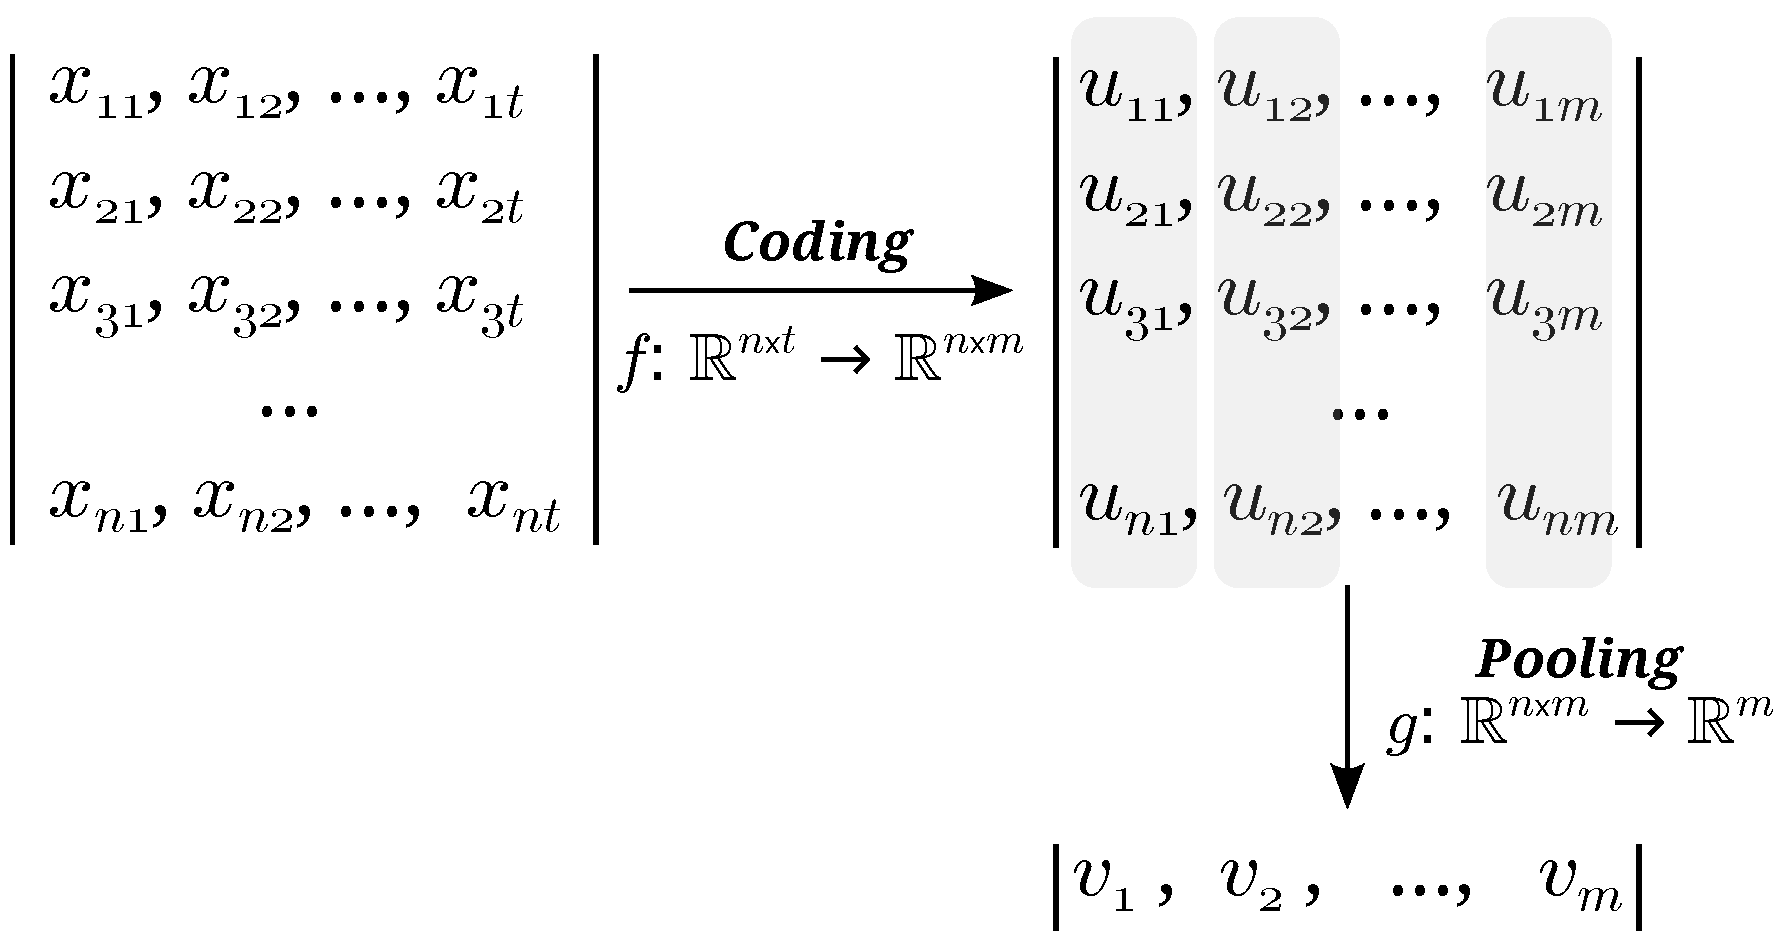
\includegraphics[width=0.48\textwidth]{coding_pooling_process.pdf}
%\caption{}
%\label{fig:coding_pooling_process}
%\end{figure}

\subsection{Classification}
After finding a new space representation for the videos in the database, we use machine learning algorithms \minor{to find} a classification model to decide whether a sample is an attempted attack or a valid access. In this paper, we evaluate the Partial Least Square (PLS)~\cite{Hoskuldsson:JC:1988} and Support Vector Machine (SVM)~\cite{Cortes:ML:1995} algorithms. 

%The PLS algorithm is a versatile data analysis tool applied in several research areas such as mathematics, economics, and computer science. PLS algorithm can be used in regression analysis, data visualization, dimensionality reduction, and data classification tasks. Similar to PCA~\cite{pearson1901lap}, the PLS is based on the linear transformation of the feature vectors to a new space formed by a small number orthogonal projection vectors. However, differently from PCA, the PLS projection vectors are chosen to maximize the covariance of the latent variables and the labels assigned to feature vectors~\cite{Schwartz:ICCV:2009}.
%
%SVM algorithm is a powerful state-of-the-art machine learning technique in many tasks of pattern recognition and computer vision. The SVM operation is based on the projection of the original space of the input feature vectors onto a higher dimensional feature space in order to find an optimal hyperplane that separates the input feature vectors into classes. SVM aims at finding the maximum margin hyperplane that separates two classes of interest. The found hyperplane can be represented as a linear combination of the input feature vectors, called support vectors, and the decision function to classify new feature vectors involves dot products between some input feature vectors. Therefore, SVM can find a separating hyperplane in the feature space and classify new feature vectors in that space without ever representing the space explicitly by means of a kernel function, which plays the role of the dot product in the feature space, avoiding explicit computations in the high dimensional feature space~\cite{James:STS:2013}.
